\documentclass[10pt,a4paper,twocolumn]{article}
\usepackage[backend=biber,style=ieee,]{biblatex}
\usepackage{tabularx}
\usepackage{amsmath}
\usepackage{graphicx} 
\addbibresource{bibliography.bib}

% Change the names
\author{
Heller, Luca\\
\and
Navaratnarajah, Suman\\
\and
Santana Martin, Irene
}
\begin{document}
\title{
    Generative Hyperparameter Optimization\\
    \large Group Assignment
}
\maketitle
\abstract{Hyperparameter Optimization (HPO) is an important way for maximizing the performance of machine learning models by testing out different hyperparameter configurations through a black-box algorithm and finding the configuration that yields the minimal loss.\\
Traditional approaches like Bayesian optimization have shown effectiveness in exploring the hyperparameter space using black-box evaluations. However, these methods often struggle with high-dimensional and complex search spaces. In this report, we propose a novel black-box optimization technique for HPO using Denoising Diffusion Probabilistic Models (DDPM), following the instructions stated by Prof. Dr. Josif Grabocka \cite{grabocka2024diffusers}. Our approach uses Bayesian optimization as the black-box optimization. In the following we will first give a brief introduction to the approach and the methods used. Secondly will go deeper into the evaluation and present our results.
\section{Introduction}
Hyperparameter Optimization (HPO) is an important process in machine learning to optimize a model given a dataset, that involves finding the optimal set of hyperparameters for a given model to achieve the best possible performance. This task is inherently challenging due to the vast and often complex hyperparameter spaces. Traditional methods such as grid search and random search are computationally expensive and inefficient. Bayesian optimization has emerged as a popular alternative, leveraging probabilistic models to make informed decisions about which hyperparameters to evaluate next. Despite its success, Bayesian optimization faces limitations when dealing with high-dimensional spaces and complex model architectures.

Recent advances in generative modeling, particularly Denoising Diffusion Probabilistic Models (DDPM), have shown promise in various domains such as image generation and natural language processing. These models learn to iteratively denoise a noisy input, gradually refining it into a coherent and high-quality output. Inspired by these advancements, we propose a novel approach to HPO that utilizes diffusion models to navigate the hyperparameter space effectively.

In this report, we detail our methodology for implementing a black-box optimization technique for HPO using diffusion models based on the instructions presented by Prof. Dr. Josif Grabocka \cite{grabocka2024diffusers}.
\section{Method} 
This method involves three main components: (1) sampling a supervised dataset from historical configurations, (2) fitting a denoising diffusion generative model, and (3) performing generative HPO search through inference with diffusion models.

To create a dataset suitable for training a diffusion model, we derive triples \((x, C, I)\) from historical data \(H\). Each triple consists of:
\begin{itemize}
  \item \(x\): Hyperparameter configuration.
  \item \(C\): Context, a set of previously evaluated configurations.
  \item \(I\): Indicator variable that shows whether the performance of \(x\) is higher than all evaluations in \(C\). Takes value 1 when performance is higher than all evaluations in C, 0 else.
\end{itemize}

The training objective for our diffusion model is to minimize the error between the expected noise and the predicted noise over \(T\) time steps.\\
$\theta^*=$ \\
$\underset{\theta}{\operatorname{argmin}} \; \mathbb{E}_{(x, I, C) \sim p_H, \; t \sim U(0, T)} \left( \epsilon_t(x) - \hat{\epsilon}_t(\hat{x}, I, C ; \theta) \right)^2$
\\
This process involves a:
\begin{itemize}
  \item \textbf{Sampler}: Randomly obtains subsets and query points from the historical data.
  \item \textbf{Noise Adder}: Adds noise to the hyperparameter configurations according to a noise schedule.
  \item \textbf{Network}: A Transformer model processes the noisy configurations and context embeddings.
  \item \textbf{Loss}: The loss function computes and minimizes the difference between the actual and predicted noise.
\end{itemize}
The trained diffusion model is used to recommend new hyperparameter configurations iteratively. For that, we need:
\begin{itemize}
  \item \textbf{Inference Process}: Using the trained DDPM to iteratively refine noisy hyperparameter configurations.
  \item \textbf{Components}:
  \begin{itemize}
    \item \textbf{Network}: Generates noise predictions for new configurations.
    \item \textbf{Denoiser}: Iteratively refines configurations by removing the predicted noise.
  \end{itemize}
\end{itemize}

\section{Evaluation}
HPO-B is a well known and used benchmark to test the implemented method. For this report, we will focus on a specific search space and experimental setting, which is given by the instructions \cite{grabocka2024diffusers}.
\vspace{5pt}
The following specifications are the ones to be used:
\begin{enumerate}
    \item [-] Meta-dataset version: "v3-test"
    \item [-] Search space: "5971"
    \item [-] Dataset: all available (”10093”, ”3954”, ”43”, ”34536”, ”9970”, ”6566”)
    \item [-] Seeds: all available ("test\_0-4")   
\end{enumerate}
We report the mean normalized regret and the according average rank for 50 trials.

\subsection{Plots}
Here is an evaluation of our method in a continuous setting and a comparison with three baselines: specifically Random Search, Gaussian Process and Deep Gaussian Process.

\begin{figure}[h]
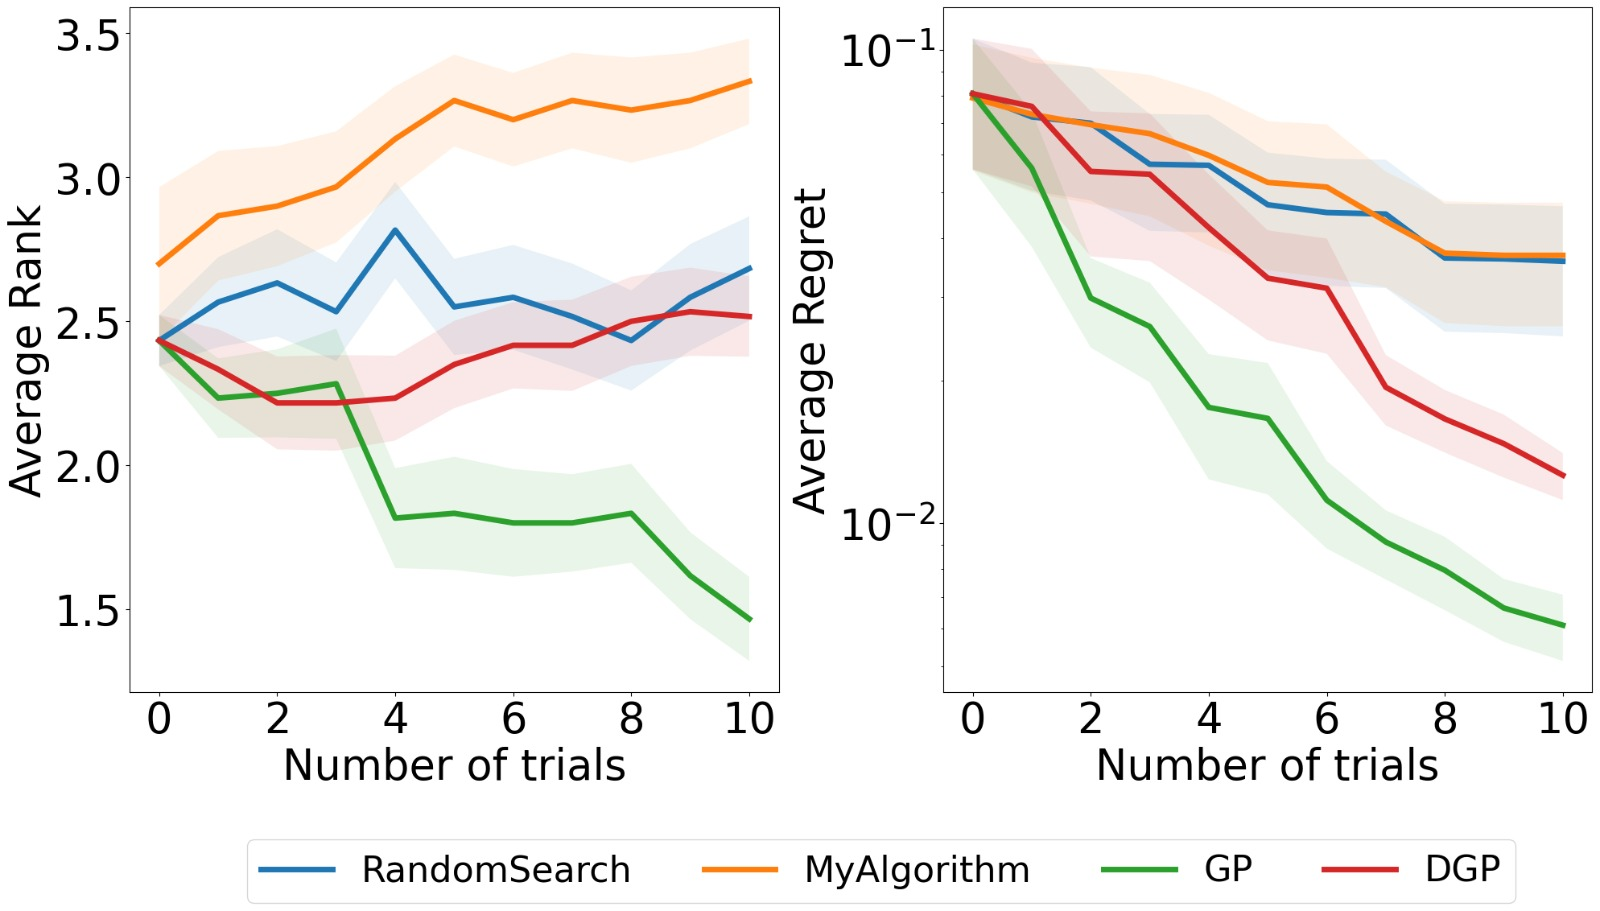
\includegraphics[width=0.5\textwidth]{img/plots.jpeg}
\caption{Our Plot: In the first upper plot, we see the "Average Rank", represented by the y-axis, against the "Number of Trials", represented by the x-axis. In the second lower plot, we see the "Average Regret", represented by the y-axis, against the "Number of Trials", represented by the x-axis.}
\label{fig:ourplot}
\end{figure}

\subsection{Approach and Challenges}
We created a repository on GitHub and distributed the tasks among the group members. Furthermore, additional issues were created in the repository for the record. We also talked to each other about our availability in order to keep in touch.

We decided to follow the steps set out in the guide. We thought it would be easy given the extensive instructions. But, it turned out to be more complicated than expected:

First, we ran into the famous problem of function-to-function dimension problems. This is a problem that we have always encountered since Machine Learning in the first semester. We were able to solve it thanks to many hours of debugging. 

Next was our lack of knowledge about the HPO benchmark, as it was the first time we worked with it. We used many hours to familiarise ourselves with it and to find out what requirements or dependencies we were missing to make everything work as expected. The README of the HPO benchmark was key, as well as several trial-and-error attempts on our own.

Finally, we had difficulty generating the plots. Because the training took so long, making small changes was more tedious than it should have been. Several times we encountered the problem that the program would suddenly stop, or at other times it would claim ‘FileNotFound’. These errors were beyond our control.

\section{Conclusion}
We got some results. Unfortunately, they were not what we had hoped for, as shown above \ref{fig:ourplot}, since it deviates a lot from what it is shown in the example from the provided guide. Lack of experience with this kind of algorithm and the HPO benchmark itself may be factors that slowed us down along the way and made us not reach our goal. Despite this, we learned a lot from this experience and are very proud of ourselves because we put a lot of effort into finishing it.

\section{Questions}
5.1. What is the mathematical formulation for the Noise Adder given the inputs in Figure 1 \cite{grabocka2024diffusers}?\\
\(x_t = \sqrt{\alpha_t x} + \sqrt{1-\alpha_t}\epsilon\) (\cite{bishop2024deeplearning}, (20.8))
\\\\5.2. What is the mathematical formulation for the Denoiser given the inputs in Figure 2 \cite{grabocka2024diffusers}?\\
\(x_{t-1} = \frac{1}{\sqrt{\alpha_t}} (x_t - \frac{1-\alpha_t}{\sqrt{1-\alpha_t}}\epsilon_t)\) (\cite{bishop2024deeplearning}, (20.35))
\\\\5.3. Do we need a transformer architecture with positional encoding? Why?\\
Yes, a transformer architecture with positional encoding is necessary. Transformers don't naturally understand the order of the input data. Positional encodings add information about the position of each element, helping the model grasp the sequence's order and relationships. (\cite{bishop2024deeplearning}, chapter 12.1.9)
\\\\5.4. Does the loss function decrease during training? Include a plot.\\
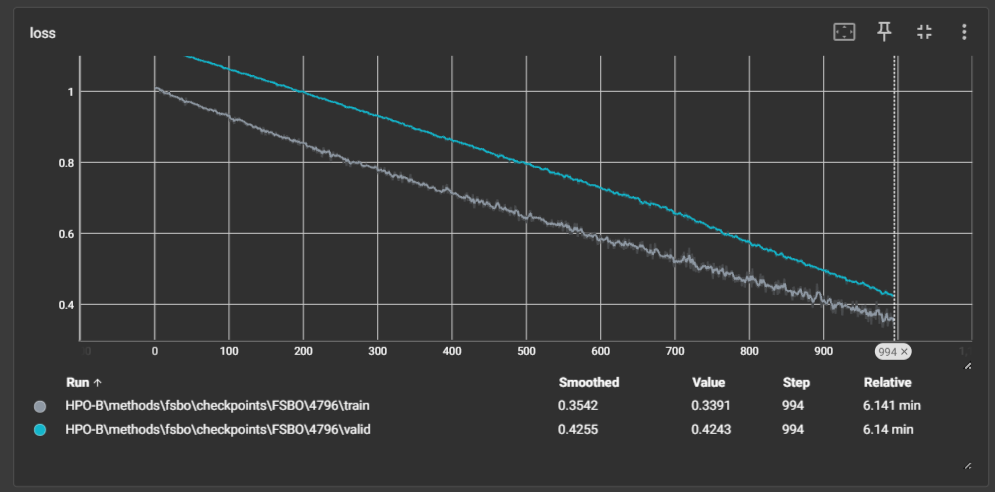
\includegraphics[width=0.5\textwidth]{img/loss.png} \\
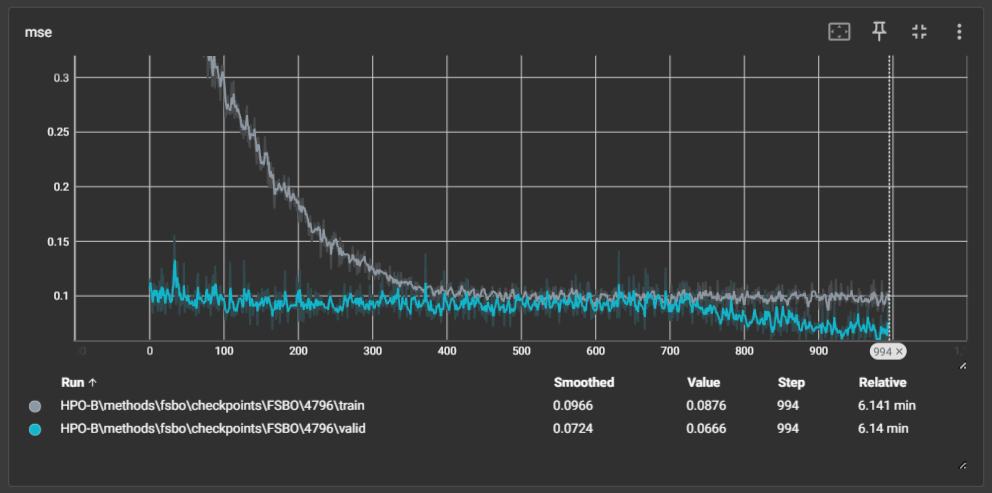
\includegraphics[width=0.5\textwidth]{img/mse.png}
\\\\5.5. What modification would you do to make the system more efficient?\\
To make training more efficient, the training should be parallelized, as the current setup (50 trials, 100 epochs and 1000 timesteps) is very slow. One could also consider using alternative sampling strategies to the current random sampling, such as rejection sampling (\cite{bishop2024deeplearning}, chapter 14.1.3), to speed up the process. 
%learning rate: we already use adam. So I guess no improvements here

\medskip
\printbibliography
\end{document}
